% !TEX encoding = UTF-8
% !TEX TS-program = pdflatex
% !TEX root = ../tesi.tex

%**************************************************************
\chapter{Progettazione e implementazione}
\label{cap:progettazione-codifica}
%**************************************************************

\intro{In questo capitolo viene descritta la progettazione dello smart contract e della sua integrazione nell'applicazione SyncTrace, per poi passare all'implementazione del contratto. Infine si analizza in modo critico lo smart contract dal punto di vista dei consumi, dando possibili alternative di implementazione.}\\

%**************************************************************

\section{Progettazione}
\begin{figure}[h]
\caption{Logo di Synctrace}
\centering

\includegraphics[width=0.5\textwidth]{./immagini/logo_synctrace}
\end{figure}
SyncTrace, il software di \textit{contact tracing} ideato dall'azienda, è formato da due applicativi. Il primo è un'applicazione mobile con cui tracciare i contatti, il secondo è una web application in cui inserire gli infetti.
Lo \textit{smart contract} da sviluppare deve fornire le funzionalità necessarie per entrambi e deve essere possibile utilizzare lo \textit{smart contract} in entrambi gli ambienti.
\subsection{Smart Contract}
Per rispettare i requisiti individuati, si è pensato di utilizzare due strutture, \textit{Person} e \textit{Contact}: \textit{Person} rappresenta una persona, mentre \textit{Contact} è un singolo contatto che una persona ha con un altro utente.\\ Il contratto \textit{Tracing} avrà poi un campo dati di tipo \textit{address} che rappresenta l'indirizzo del proprietario del contratto, una mappa che associa l'id di una persona alla struttura \textit{Person} e una mappa che associa l'id di una persona a un \textit{array} di contatti registrati.
La figura \hyperref[fig:umlcontract]{4.2} riporta un piccolo diagramma riassuntivo che rappresenta lo \textit{smart contract} Tracing, con le varie funzionalità richieste dai requisiti.
\begin{figure}[h]
\label{fig:umlcontract}
\caption{Diagramma \emph{\gls{UML}}\glsfirstoccur smart contract}
\centering
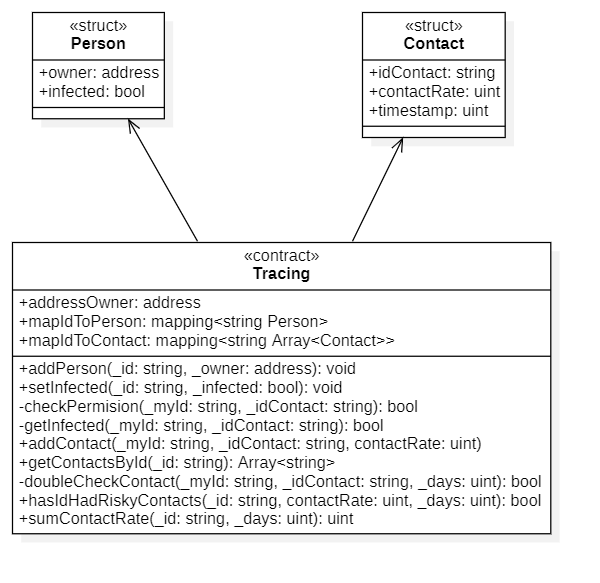
\includegraphics[width=0.75\textwidth]{./immagini/tracingcontractuml}
\end{figure}
\FloatBarrier

Come si può notare dal diagramma, \textit{Person} ha due campi dati:
\begin{itemize}
	\item{\textit{address owner}: indica l'account Ethereum di ogni persona, necessario per permettere l'utilizzo delle funzionalità solo sul proprio account;}
	\item{\textit{bool infected}: booleano che indica lo stato di salute della persona.}
\end{itemize}
Contact invece ha:
\begin{itemize}
	\item{\textit{string idContact}: indica l'id della persona con cui si è entrati in contatto;}
	\item{\textit{uint contactRate}: indica l'indice di contatto avuto, calcolato in base al tempo e alla distanza;}
	\item{\textit{uint timestamp}: indica il momento in cui è stato registrato il contatto.}
\end{itemize}

Una volta effettuato il \emph{\gls{deployment}}\glsfirstoccur, il contratto Tracing deve inizializzare \textit{addressOwner} con l'indirizzo dell'account che ha effettuato il deployment, ossia l'account dell'azienda. Questo account avrà dei privilegi attraverso i quali sarà possibile utillizzare delle funzioni critiche. Per esempio la funzione per segnalare un infetto non deve poter essere chiamata da chiunque, per scongiurare la possibilità che qualcuno possa segnalarsi infetto, anche se non lo è.\\
La mappa che contiene le persone registrate è stata pensata per essere popolata al primo avvio dell'applicazione con un id generato randomicamente.\\
I contatti di ogni persona, invece, saranno aggiunti ogni volta che l'applicazione rileva un contatto tramite la tecnologia bluetooth LE.

\subsection{Integrazione mobile}
Per sfruttare la rete \textit{Ethereum} in android si utilizza la libreria \textit{Java web3j}, nata per lavorare con gli smart contract e interagire con i nodi di \textit{Ethereum}
\begin{figure}[h]
\caption{Integrazione applicazione Java - client Ethereum con web3j}
\centering
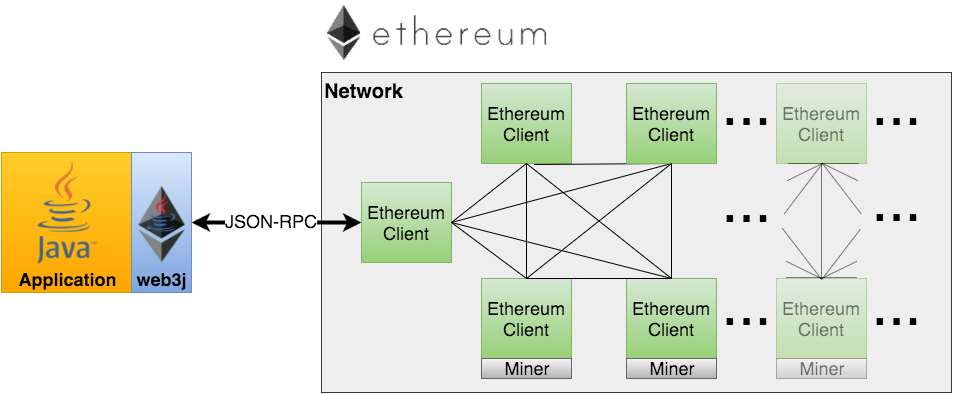
\includegraphics[width=0.8\textwidth]{./immagini/web3j_network.png}
\end{figure}
\FloatBarrier
La figura \hyperref[fig:umlapp]{4.4} riporta un diagramma \textit{uml} che mostra l'integrazione del contratto con l'applicazione mobile SyncTrace.
A partire dal contratto Tracing, grazie a \textit{web3j}, si genera una classe Java \textit{TracingContract} che contiene le funzioni dello \textit{smart contract}, oltre a due metodi per effettuare il \textit{deployment} e il caricamento del contratto.
La classe \textit{TracingContract} viene a sua volta utilizzata da un \textit{BlockchainManager}, che gestisce la configurazione e tutte le operazioni necessarie all'applicazione.
In questo modo, quando nel codice dell'applicazione è necessario effettuare una chiamata allo \textit{smart contract}, è sufficiente instanziare la classe \textit{BlockchainManager} e chiamare il metodo desiderato.
I dettagli relativi all'implementazione nell'applicazione saranno discussi approfonditamente in seguito.

\begin{figure}[h]
\label{fig:umlapp}
\caption{Diagramma di classe integrazione smart contract - SyncTrace app}
\centering
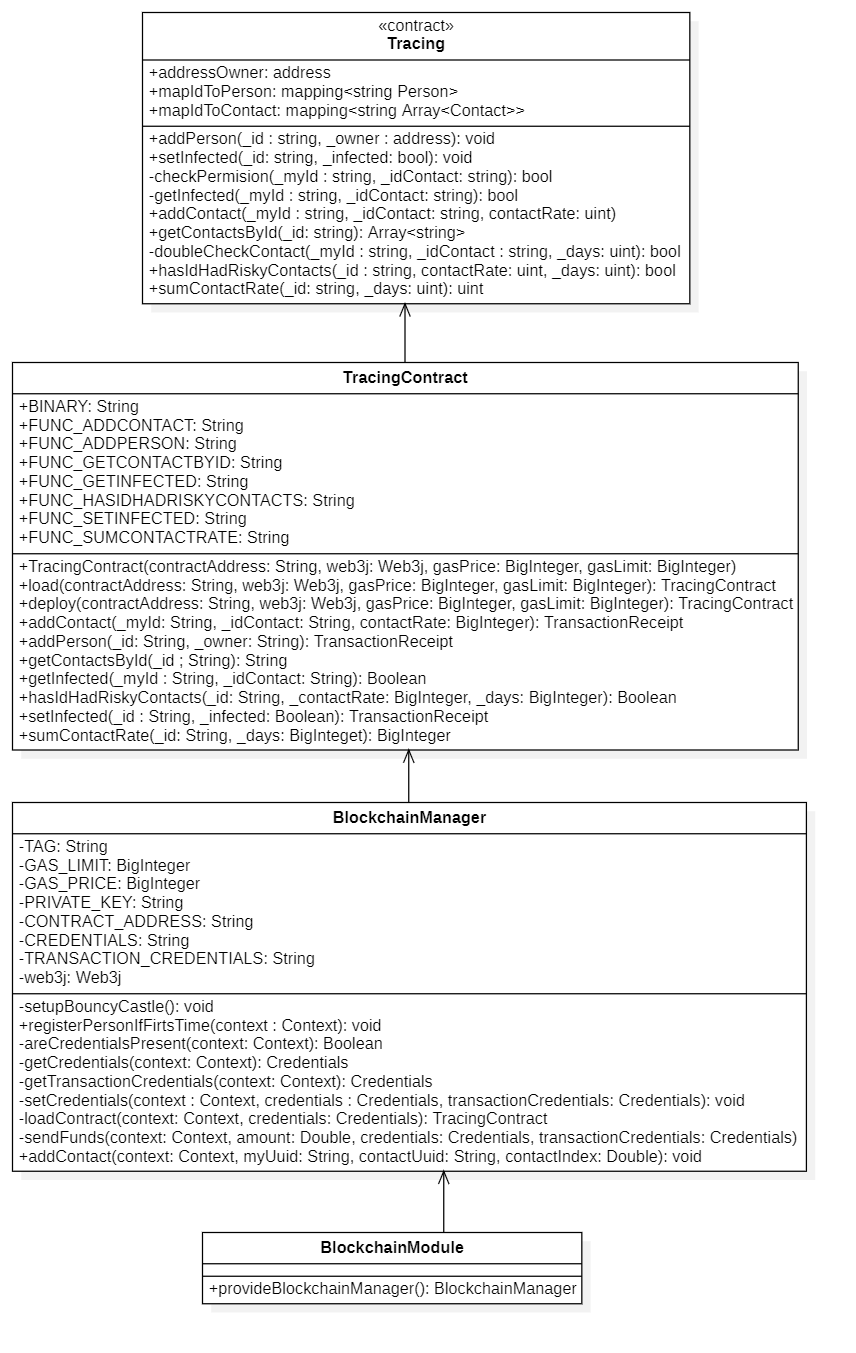
\includegraphics[width=0.76\textwidth]{./immagini/tracinguml.png}
\end{figure}

\FloatBarrier

\subsection{Integrazione web application}
Come nell'ambiente mobile, anche per la web application si utilizza una libreria per interagire con \textit{Ethereum}: \textit{web3js}. 
Per integrare lo \textit{smart contract} alla web app di SyncTrace è sufficiente implementare uno script che configuri la connesione al nodo della \textit{blockchain} e richiami la funzione dello \textit{smart contract} adibita all'inserimento di una persona infetta.
Nel capitolo 5 verrà approfondita la questione.

\subsection{Diagramma di sequenza}
Per comprendere il funzionamento generale di SyncTrace con la \textit{blockchain} riporto un diagramma di sequenza semplificato che mostra come le parti interagiscano nel caso d'uso principale:

\begin{figure}[h]
\caption{Diagramma di sequenza SyncTrace}
\centering
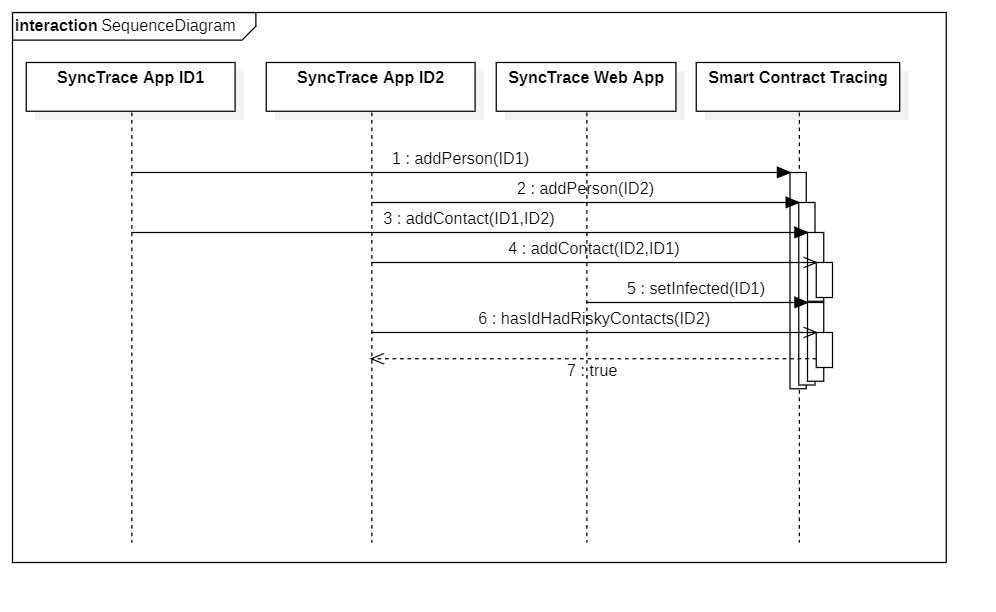
\includegraphics[width=1.0\textwidth]{./immagini/sequenza.png}
\end{figure}

Nel diagramma sono presenti quattro partecipanti: due applicazioni SyncTrace mobile, la web application di SyncTrace e lo \textit{smart contract}.
Quando l'applicazione viene installata negli smartphone, vengono create delle credenziali e l'utente viene aggiunto in catena con il metodo \textit{addPerson}.
Il diagramma, poi, mostra l'aggiunta di un contatto tra le due applicazioni tramite la funzione \textit{addContact}.\\ 
Quando una persona risulta positiva a un tampone, tramite web application, è possibile segnalare il suo stato di salute con la funzione \textit{setInfected}.\\
A questo punto, l'applicazione che ha registrato un contatto con il malato, interrogando la\textit{blockchain} con il suo identificativo, otterrà il valore booleano \textit{true}, che indica che tra i suoi contatti è presente un infetto.


\section{Proof of concept}
Prima di mostrare lo smart contract sviluppato, ritengo utile mostrare una versione inizialmente pensata con il tutor aziendale e implementata come \emph{\gls{Proof of concept}}\glsfirstoccur, per analizzare le differenze tra i due contratti, soprattutto come consumi di gas. Una parte dello stage, infatti, è stata incentrata su come ottimizzare il codice \textit{Solidity}, cercando di progettare lo \textit{smart contract} in modo da raggiungere i requisiti con le operazioni meno onerose nella piattaforma \textit{Ethereum}.
Le funzionalità di questa versione del contratto sono le medesime di quello definitivo e, per questo, non verranno illustrate in questa sezione.
Il codice riportato nelle prossime righe mostra la differenza nelle struct e nei campi dati del contratto rispetto alla progettazione definitiva.

\mbox{\newline}
\begin{lstlisting}[language=Solidity]
pragma solidity ^0.6.7;
pragma experimental ABIEncoderV2;

contract Tracing {

    struct Person {
        string id;
        address owner;
        bool infected;
    }

    struct Contact{
        Person p1;
        Person p2;
        uint256 contactRate;
        uint256 timestamp;
    }

    contract Tracing {
    
        address ownerAddress;
        Person[] people;
        Contact[] contacts;

	/*
		methods
	*/
}

\end{lstlisting}
\mbox{\newline}
Come per la versione definitiva, sono presenti le due struct \textit{Person} e \textit{Contact}, ma con alcune differenze.
\textit{Person} contiene anche l'id dell'utente, mentre \textit{Contact} ha due campi dati \textit{Person} che rappresentano gli utenti entrati in contatto.
Per quanto riguarda i campi dati del contratto, è sempre presente un address con lo stesso scopo, ma il modo di registrare le persone e i contatti è differente. Invece di usare delle mappe sono presenti due \textit{array}, rispettivamente \textit{people} e \textit{contacts}. Lo scopo dell'\textit{array} \textit{people} è sostanzialmente lo stesso della mappa \textit{mapIdToPerson}, ovvero contenere tutti gli utenti registrati. Per registrare i contatti, invece, c'è una grande differenza di progettazione. Invece di associare ogni persona a un'\textit{array} che contenga tutti i contatti che ha, è presente un unico \textit{array contacts}, che include tutti i contatti avuti tra gli utenti.\\
Il \textit{Proof of concept} mostrato è stato scartato per alcune criticità. In primo luogo avere una struttura dati che contenga i contatti di tutti gli utenti non è una soluzione particolarmente furba perché complica inutilmente il contratto in qualsiasi tipo di operazione sui contatti e, soprattutto, perché per il suo funzionamento sono richieste operazioni particolarmente onerose per quanto riguarda il consumo di gas, come il confronto tra stringhe. Infatti in \textit{Solidity} non è supportato il confronto booleano tra due stringhe. Per bypassare questo problema è necessario calcolare l’\textit{hash} delle due stringhe e poi confrontarlo. Il calcolo dell’\textit{hash}, però, è una delle operazioni più onerose in \textit{Ethereum}.\\
Nella sezione \hyperref[sec:gas]{4.3.2} approfondirò l’argomento, mostrando i consumi del \textit{proof of concept} a confronto con il contratto definitivo.

\section{Implementazione}
\subsection{Smart contract Tracing}
L'implementazione dello \textit{smart contract}, come visto nella sezione progettazione, prevede l'utilizzo di due strutture, un address e due mappe per associare l'id di un utente alle sue informazioni e ai suoi contatti.
L'intestazione del contratto, dunque, è la seguente:

\mbox{\newline}
\begin{lstlisting}[language=Solidity]
pragma solidity ^0.6.7;
pragma experimental ABIEncoderV2;

contract Tracing {

    struct Person {
        address owner;
        bool infected;
    }

    struct Contact {
        bytes32 idContact;
        uint256 contactRate;
        uint256 timestamp;
    }
    
    address ownerAddress;
    mapping(bytes32 => Person) mapIdToPerson;
    mapping(bytes32 => Contact[]) mapIdToContact;

	/*
	methods
	*/
}

\end{lstlisting}
È disponibile un costruttore che al momento del \textit{deployment} assegna la variabile \textit{addresOwner} al chiamante \textit{msg.sender}:

\mbox{\newline}
\begin{lstlisting}[language = Solidity]

    constructor() public {
        ownerContract = msg.sender;
    }

\end{lstlisting}
\mbox{\newline}

Inoltre viene dichiarato un modificatore che viene utilizzato da diverse funzioni del contratto.
In \textit{Solidity} un modificatore viene eseguito prima della funzione in cui ne viene richiesto l'utilizzo. Come un metodo, ha un nome e degli argomenti, e al suo interno si trova una condizione. Se la condizione è soddisfatta, viene eseguito il corpo della funzione che utilizza il modificatore; in caso contrario la funzione non viene eseguita.\\
Nel \textit{contract Tracing} la condizione del modificatore \textit{isOwner} è di eseguire la funzione se e solo se l'utente che chiama il metodo ha l'address che corrisponde a quello salvato nel campo dati \textit{owner} della persona con id dato in input. In questo modo le funzioni in cui viene specificata questa condizione possono essere eseguite solo da chi ha i permessi per farlo. Il modificatore è il seguente:

\mbox{\newline}
\begin{lstlisting}[language = Solidity]

    modifier isOwner(bytes32 _id) { 
        require(msg.sender == mapIdToPerson[_id].owner,"You are not the owner");
        _; 
    }

\end{lstlisting}
\mbox{\newline}

Sono state implementate delle funzioni ad uso interno, ossia non visibili e non eseguibili se non all'interno dello \textit{smart contract}.
Sono funzioni di utilità utilizzate da alcuni metodi pubblici e per questo non sono disponibili all'utente:

\mbox{\newline}
\begin{lstlisting}[language = Solidity]

/*
Funzione di utilita' che prende in input l'id di chi chiama la funzione e l'id del contatto da verificare.
Prima dell'esecuzione chiama il modificatore isOwner per verificare i permessi.
Ritorna il valore del booleano infected per la persona di id = _idContact
*/
function getInfected(bytes32 _myId,bytes32 _idContact) internal view isOwner(_myId) returns (bool);

/*
Funzione di utilita' che prende in input l'id di chiama la funzione, l'id del contatto da verificare e il numero dei giorni da controllare.
Verifica che se il primo id ha aviuto un contatto con il secondo id, anche il secondo id deve aver avuto un contatto con il primo.
Ritorna un booleano che indica il risultato del controllo
*/
function doubleCheckContact(bytes32 _myId, bytes32 _idContact,uint _days) internal view returns (bool);

\end{lstlisting}
\mbox{\newline}

Infine le funzioni disponibili all'utente hanno tutte come visibilità \textit{external} e sono le seguenti:

\mbox{\newline}
\begin{lstlisting}[language=Solidity]
/*
Funzione che prende in input l'id e l'indirizzo di una persona e l'aggiunge alla mappa mapIdToPerson.
Se la persona e' gia' presente nella mappa, viene restituito un errore.
*/
function addPerson(bytes32 _id, address _owner) external;

/*
Funzione che prende in input l'id di una persona e un booleano che indica il suo stato di salute (infetto o meno). e cambia la variabile infected della persona con l'id inserito. 
Puo' essere chiamata solo dall'account proprietario del contratto (chi ha fatto il deployment)
Restituisce un errore se l'id non e' registrato.
*/    
function setInfected(bytes32 _id,bool _infected) external;

/*
Funzione che prende in input l'id del chiamante, l'id del contatto avuto e un indice di contatto.
Aggiunge un contatto con i dati in input alla mappa mapIdToContacts.
Restituisce un errore se il chiamante non ha i permessi per inserire il contatto o se gli id inseriti non sono registrati.
*/    
function addContact(bytes32 _myId,bytes32 _idContact,uint _contactRate) external isOwner(_myId);

/*
Funzione che prende in input un id e restituisce un array contenente i contatti dell'id inserito.
Restituisce un errore se il chiamante non ha i permessi per richiedere i contatti oppure se l'id inserito non e' registrato.
*/    
function getContactsById(bytes32 _id) external view isOwner(_id) returns(bytes32[] memory);

/*
Funzione che prende in input un id, un indice di contatto e un numero di giorni.
Controlla se tra i contatti della persona con l'id inserito ci sia un contatto con una persona infetta.
Il contatto deve avere indice superiore a quello indicato e deve essere avvenuto negli ultimi giorni inseriti in input.
Restituisce un errore se il chiamante non ha i permessi necessari.
*/    
function hasIdHadRiskyContacts(bytes32 _id,uint _contactRate,uint _days) external view isOwner(_id) returns (bool);

\end{lstlisting}
\newpage
\begin{lstlisting}[language=Solidity]
/*
Funzione che prende in indice un id e un numero di giorni.
Ritorna la somma degli indici di contatto per l'id in input negli ultimi giorni indicati.
Restituisce un errore se il chiamante non ha i permessi necessari.
*/   
function sumContactRate(bytes32 _id,uint256 _days) external view isOwner(_id) returns (uint256);

\end{lstlisting}

\mbox{\newline}

\subsection{Analisi gas}
\label{sec:gas}
In \textit{Ethereum} ogni operazione effettuata, che cambia lo stato della \textit{blockchain}, consuma gas. Il gas è un’unità di misura utilizzata per pagare la computazione effettuata dai \textit{miner}. Più un'operazione è dispendiosa a livello di risorse, più gas questa operazione costa.
Il concetto di gas permette di addebitare una tariffa che viene pagata ai \textit{miner}, incentivandoli a prendere parte attiva al sistema.\\
Tuttavia, il gas rappresenta un cambio di paradigma rispetto alla programmazione classica. Non sempre un approccio vantaggioso in un normale linguaggio di programmazione rappresenta la \textit{best practice} in \textit{Solidity}, proprio perché c’è una variabile in più da considerare. 
Nel corso dello stage è stata rivolta particolare attenzione a questo aspetto: il \textit{contract} è stato ottimizzato per cercare di limitare il più possibile il consumo di gas.\\

Dal \textit{Proof of concept} allo \textit{smart contract} finale, infatti, la differenza di gas per il \textit{deployment} e per le operazioni è notevole. Nelle tabelle successive sono riporatati i consumi per entrambe le versioni. I costi stimati in euro fanno riferimento all'attuale tasso di conversione di 202 euro/ether. Il costo per unità di gas, invece è 26 \emph{\gls{gwei}}\glsfirstoccur/gas.
\newpage
\begin{center}
	\begin{longtable}{| c | c | c |}
		\caption{Tabella gas Proof of Concept}
		\label{tab:gas-poc}\\
		\hline
		\textbf{Metodo} & \textbf{Consumo gas medio} & \textbf{Costo medio (eur)}\\
		\endfirsthead
		\hline
		\textbf{Metodo} & \textbf{Consumo gas medio} & \textbf{Costo medio (eur)}\\
		\endhead
		\textbf{Deployment} & \textbf{1599579} & \textbf{8.41}\\
		\hline
		\endfoot
		
		\hline
		addPerson & 79367 & 0.41\\
		\hline
		addContact & 203512 & 1.07\\
		\hline
		setInfected & 50111 & 0.26\\
		\hline
	\end{longtable}
\end{center}

\begin{center}
	\begin{longtable}{| c | c | c |}
		\caption{Tabella gas Tracing}
		\label{tab:gas-tracing}\\
		\hline
		\textbf{Metodo} & \textbf{Consumo gas medio} & \textbf{Costo medio (eur)}\\
		\endfirsthead
		\hline
		\textbf{Metodo} & \textbf{Consumo gas medio} & \textbf{Costo medio (eur)}\\
		\endhead
		\textbf{Deployment} & \textbf{839416} & \textbf{4.41}\\
		\hline
		\endfoot
		
		\hline
		addPerson & 43859 & 0.23\\
		\hline
		addContact & 104806 & 0.55\\
		\hline
		setInfected & 29364 & 0.15\\
		\hline
	\end{longtable}
\end{center}

Come si può notare, il costo del \textit{deployment} dei due \textit{smart contract} è quasi dimezzato: 1.600.000 contro 830.000. Il risparmio c'è, ma non è il più significativo pensando al fatto che il \textit{deployment} viene effettuato una singola volta. Il costo del \textit{deployment}, in un'applicazione \textit{Ethereum}, è abbastanza marginale rispetto al costo delle operazioni se, come in questo caso, le funzioni devono essere chiamate molte volte.
Risulta molto più interessante analizzare il consumo delle funzioni \textit{addPerson}, \textit{addContact} e \textit{setInfected}. Anche per queste operazioni il risparmio è molto importante: ogni chiamata ha un consumo all'incirca dimezzato rispetto al \textit{Proof of Concept}:
\begin{itemize}
\item{\textit{addPerson}: 79367 prima, 43859 dopo}
\item{\textit{addContact}: 203512 prima, 104806 dopo}
\item{\textit{setInfected}: 50111 prima, 29364 dopo}
\end{itemize}

Questi risultati sono in parte dovuti alla modifica progettuale del contratto. Nel \textit{Proof of Concept} sono stati utilizzati \textit{array} dinamici per contenere gli utenti registrati e i contatti. Al contrario, nello \textit{smart contract} finale, si è fatto uso di mappe. In \textit{Solidity} gli array dinamici hanno delle \textit{features} che li rendono inevitabilmente più costosi come: 
\begin{itemize}
\item{La variabile \textit{length}, per contare il numero di oggetti memorizzati;}
\item{Il \textit{bound-checking} per avere un controllo sull'accesso casuale.}
\end{itemize}

Inoltre, grazie all'utilizzo delle mappe, le funzioni dello \textit{smart contract} risultano essere più semplici e con meno operazioni da effettuare. Un esempio lampante è il confronto tra stringhe. Per la natura del contratto, nel \textit{Proof of concept} è necessario confrontare più volte gli id di tipo stringa. Il confronto booleano tra stringhe, però, non esiste in \textit{Solidity}. Si può risolvere questa problematica calcolando l'\textit{hash} delle stringhe, per poi confrontare il risultato. Tuttavia, l'operazione di \textit{hashing} è una tra le più onerose e aumenta sensibilmente il costo del contratto.\\

Sono stati presi altri accorgimenti per il risparmio di gas come:
\begin{itemize}
\item{\textbf{Funzioni interne: }è stata utilizzzata la visibilità internal per le funzioni non utilizzate all'esterno del contratto;}
\item{\textbf{Funzioni esterne: }è stata utilizzata la visibilità external invece di quella public;}
\item{\textbf{Storage: }sono state limitate le operazioni di storage;}
\item{\textbf{Eventi: }gli eventi non sono stati utilizzati. Le funzioni che emettono eventi hanno un costo molto superiore;}
\item{\textbf{Tipo bytes: }dove possibile è stato utilizzato il tipo bytes invece del tipo stringa;}
\item{\textbf{Assert vs require: }le eccezioni sono state gestite con la keyword require;}
\item{\textbf{Ottimizzazione compilazione: }la compilazione Solidity è stata ottimizzata con la keyword optimize;}
\end{itemize}

\subsection{Fattibilità applicazione reale}
Anche con la massima efficienza di uno smart contract, è fondamentale considerare il caso d’uso dell’applicazione, per rendersi conto della fattibilità del progetto.
Come accennato prima, i costi maggiori in \textit{Ethereum} non sono rappresentati dal \textit{deployment} del contratto, bensì dal numero di chiamate stimate alle funzioni che consumano gas.
Nel nostro caso d’uso, la funzione \textit{addPerson} viene eseguita ogni qualvolta una persona installa l’applicazione nel proprio smartphone. Considerando come campione metà della popolazione italiana, il metodo viene chiamato 30 milioni di volte. Con il prezzo attuale dell'\textit{Ether} (202 euro/Ether) e impostando il \textit{gas price} a 26 gwei/gas, ogni chiamata costa circa 23 centesimi. Questo vuol dire che solo per l’installazione il costo stimato è di 7,5 milioni di euro.
Già questo piccolo calcolo sarebbe sufficiente per rendersi conto che questo \textit{smart contract} non è sostenibile in un contesto di utilizzo reale. Purtroppo però, c’è una spesa ancora maggiore. In \textit{blockchain} viene inserito ogni contatto superiore a 15 minuti, a distanza inferiore di 2 metri, per ogni persona che ha l’applicazione. Con il \textit{gas price} e il tasso di cambio indicati, la chiamata per aggiungere un contatto ha un costo di circa 50 centesimi e non è difficile immaginare che il numero di chiamate sia di svariati milioni al giorno. Per questo motivo, soluzioni di questo genere sono difficilmente utilizzabili nella realtà.
Tuttavia ci sono delle soluzioni alternative.
\\
\subsection{Soluzioni}
\subsubsection{Smart contract semplificato}
Come detto, in \textit{Ethereum}, la soluzione proposta non è realizzabile nella pratica. Una possibile alternativa nell’ambito contact tracing è rappresentata dalla gestione locale di tutti i contatti tra le persone. Ogni dispositivo mobile possiede un id; i contatti con gli altri dispositivi vengono registrati e salvati localmente. Ogni 14 giorni vengono eliminati perché considerati ininfluenti per il contagio.
Quando una persona viene trovata infetta a seguito di un tampone, il medico (sotto autorizzazione del contagiato) lo segnala tramite web app. A seguito di questa segnalazione, l’id del malato viene inserito nell’\textit{array} degli infetti nello \textit{smart contract}. 
In questo modo lo \textit{smart contract} risulta estremamente più semplice. Gestisce un \textit{array} di infetti con una funzione per l'aggiunta e una per la rimozione, in modo sicuro e immutabile.
Lo smart contract in questione potrebbe essere implementato in questo modo:

\mbox{\newline}
\begin{lstlisting}[language = Solidity]
pragma solidity ^0.6.7;
pragma experimental ABIEncoderV2;

contract Tracing {

    bytes32[] infected;
    
    function addInfected(bytes32 _id) external {
        //require only doctors
        infected.push(_id);
    }

    function removeInfected(bytes32 _id) external {
        //require only doctors
        for(uint i = 0; i < infected.length; i++) {
            if(infected[i] == _id) {
                infected[i] = infected[infected.length - 1];
                infected.pop();
            }
        }
    }  
    
    function getInfected() external view returns (bytes32[] memory){   
        uint length = 0;
        for(uint i = infected.length; i > 0; i--) {
            length++;
        }
        bytes32[] memory toReturn = new bytes32[](length);
        for(uint i = infected.length; i > 0; i--) {
            toReturn[i-1] = infected[i-1]; 
        }
        return toReturn;
    }
   
}
\end{lstlisting}
\mbox{\newline}

Lato mobile, periodicamente il dispositivo chiama la funzione dello \textit{smart contract} che restituisce gli infetti. Gli id ritornati vengono confrontati con gli id dei contatti salvati localmente per verificare la presenza di un rischio contagio.
Tutte le altre operazioni sono effettuate localmente. Il consumo del gas è infinitamente più contenuto e permette un utilizzo reale dell’applicazione. Questo perché le uniche operazione che richiedono una transazione, e dunque un consumo di gas, sono quelle di inserimento e rimozione di un id nell’\textit{array}. Questi metodi possono essere eseguiti solo dal personale sanitario a seguito di un tampone risultato positivo. \\
Il consumo di gas per questo \textit{smart contract} è riportato nella seguente tabella:
\begin{center}
	\begin{longtable}{| c | c | c |}
		\caption{Tabella gas smart contract semplificato}
		\label{tab:gas-simplytracing}\\
		\hline
		\textbf{Metodo} & \textbf{Consumo gas medio} & \textbf{Costo medio (eur)}\\
		\endfirsthead
		\hline
		\textbf{Metodo} & \textbf{Consumo gas medio} & \textbf{Costo medio (eur)}\\
		\endhead
		\textbf{Deployment} & \textbf{196237} & \textbf{1.04}\\
		\hline
		\endfoot
		
		\hline
		addInfected & 52272 & 0.28\\
		\hline
		removeInfected & 28353 & 0.15\\
		\hline
	\end{longtable}
\end{center}

Dalla tabella si può notare come il costo di \textit{deployment} del contratto sia notevolmente inferiore rispetto al precedente: 1.500.000 gas contro 200.000 circa. 
Ma la differenza la fa soprattutto il numero di chiamate alle funzioni \textit{addInfected} e \textit{removeInfected}, decisamente inferiori rispetto a tutte le chiamate necessarie per registrare i contatti.
In Italia i contagi certificati ad oggi sono circa 200 mila. Considerando un costo di circa 20 centesimi a chiamata per ogni infetto, supponendo anche che tutti gli infetti siano registrati all’applicazione e diano il consenso al proprio medico, la spesa totale dell’utilizzo del contratto si aggirerebbe intorno a 40 mila euro, in linea con le \textit{dApp} più utilizzate. \\
\subsubsection{Altre blockchain}
Un’altra soluzione, che può essere anche complementare a quella appena descritta, prevede un cambio di piattaforma. \textit{Ethereum} infatti, nonostante sia la \textit{blockchain} più diffusa per lo sviluppo di \textit{applicazioni decentralizzate}, ha un costo molto alto e destinato ad aumentare con l’aumentare degli utenti.
Questo è dovuto all’algoritmo di consenso che \textit{Ethereum}, come la maggiorparte delle \textit{blockchain}, utilizza attualmente, ossia il \textit{proof of work}. La computazione richiesta per validare i blocchi e le transazioni richiedono il pagamento di una \textit{fee}, proporzionale alle risorse richieste. 
Tuttavia, esistono altri tipi di \textit{blockchain} che utilizzano il consenso \textit{proof of stake}, come la piattaforma EOS.
La scalabilità e le transazioni gratuite sono i punti di forza di EOS. Il processo non è comunque gratuito, ma richiede che l’utente possieda un numero di \textit{token (stake)} che gli permetta di “affittare” le risorse necessarie per validare le transazioni. Questi \textit{token}, però, non sono spesi, ma possono essere restituiti quando desiderato al prezzo corrente della criptovaluta.
Anche \textit{Ethereum} sta effettuando il passaggio al \textit{proof of stake}, con la piattaforma che verrà denominata \textit{Ethereum 2.0}, in arrivo a fine 2020. 
Il passaggio definitivo, con la chiusura di \textit{Ethereum 1.0} è previsto per il 2022.
\textit{Ethereum 2.0} è molto atteso perché il \textit{proof of stake} cambia completamente il modo di vedere le \textit{blockchain}. La scalabilità è uno dei problemi maggiori delle \textit{blockchain} che si basano su \textit{proof of work}, limitandone possibili applicazioni. Con \textit{Ethereum 2.0}, invece, potrebbe essere possibile utilizzare le \textit{blockchain} per qualsiasi tipo di \textit{applicazione decentralizzata}, senza accusare differenze rispetto a quelle tradizionali.

\section{Test smart contract}
I test dello \textit{smart contract} sono stati fatti con il linguaggio JavaScript sfruttando la \textit{suite truffle}.
Di seguito è riportata la tabella di tracciamento dei test.

\begin{center}
	\begin{longtable}{| c | p{25em} | c |}
		\caption{Tabella test smart contracti}
		\label{tab:test-sci}\\
		\hline
		\textbf{Test id} & \centering\textbf{Descrizione} & \textbf{Requisiti coperti}\\
		\endfirsthead
		\hline
		\textbf{Test id} & \centering\textbf{Descrizione} & \textbf{Requisiti coperti}\\
		\endhead
		\endfoot
		
		\hline
		UT-1     & Should deploy smart contract properly and save owner address & RFN-1 \\
		\hline
		UT-2     & Should add two person to people array and get them by id & RFN-2 - RF10\\
		\hline
		UT-3     & Should not be able to add the same id person in people array & RFN-3 \\
		\hline
		UT-4     & Should add a contact between two id presents in people array & RFN-7 \\
		\hline
		UT-5     & Should not be able to add another person contacts & RFN-8 \\
		\hline
		UT-6     & Should not be able to add a contact with nonexisting person & RFN-9 \\
		\hline
		UT-7     & Should set a person infected & RFN-4 \\
		\hline
		UT-8     & Should not be able to set a person infected if the address is not who deploys the contract & RFN-5 \\
		\hline
		UT-9     & Should not be able to set infected a nonexisting person & RFN-6 \\
		\hline
		UT-10   & Should not be able to get other people contacts & RFN-11 \\
		\hline
		UT-11   & Should check that the second id has a infection risk & RFN-12 \\
		\hline
		UT-12   & Should check that if a contact is not confirmed, then a person has not risk infection &  13\\
		\hline
		UT-13   & Should not be able to check another person risk infection & RFN-14 \\
		\hline
		UT-14   & Should check that sum of contactRates in the last day is 15 for the first id & RFN-15 \\
		\hline
		UT-15   & Should not be able to calculate another person sum of contactRates & RFN-16 \\
		\hline
	\end{longtable}
\end{center}
